\documentclass[12pt,a4paper]{book}
\usepackage[utf8]{inputenc}
\usepackage{amsmath}
\usepackage{amsfonts}
\usepackage{amssymb}
\usepackage{graphicx}
\usepackage[polish]{babel}
\usepackage{polski}
\usepackage{authoraftertitle}
\usepackage{geometry}
\usepackage{graphicx}

\newgeometry{tmargin=2.5cm, bmargin=2.5cm, lmargin=2.5cm, rmargin=2.5cm}
\setcounter{secnumdepth}{0}
\setlength\parindent{0pt}


\pagestyle{plain}
\title{Wielka Kołowa Księga Kucharska}
\author{Koło Matematyków Studentów UJ im. prof. Stanisława Zaremby}
\date{2020}

\begin{document}
	\begin{titlepage}
		\begin{center}
			\vspace*{200pt}
			{\huge\bfseries \MyTitle}\\
			% ----------------------------------------------------------------
			\vspace{1.5cm}
			\textsc{\Large{{Koło Matematyków Studentów UJ\\im. prof. Stanisława Zaremby}}} \\[5pt]
			\vfill
			{\the\year}
		\end{center}
	\end{titlepage}

	\tableofcontents
	
	\part{Przystawki}

\section{Przykładowy przepis}
\vspace*{8pt}

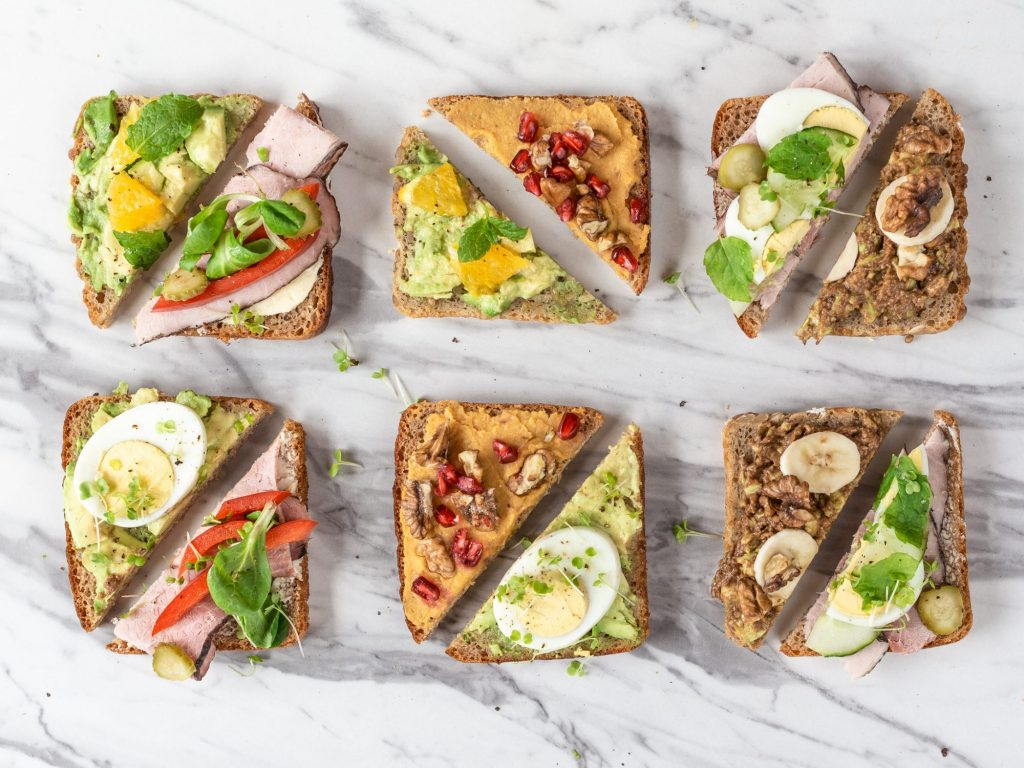
\includegraphics[width=\linewidth]{przystawki/img/kanapki}
\vspace{2pt}

\textit{Czas przygotowania: 5 minut}\\
\textit{Porcja dla 2 osób}\\

\vspace{2pt}

Składniki:
\begin{itemize}
	\item składnik 1 (200 g),
	\item składnik 2 (250 ml),
	\item składnik 3 (1 szt.),
	\item składnik 4,
	\item dodatek 1.
\end{itemize}

Lorem ipsum dolor sit amet, consectetur adipiscing elit. Fusce sed nisi malesuada, luctus dolor ut, semper nisi. Morbi feugiat massa urna, at aliquam sapien euismod vitae. Sed id nisi ac purus aliquam sollicitudin. Morbi sed consequat lorem, in dignissim nulla. Curabitur ut ipsum aliquam, ornare sem eu, cursus nisl. Mauris commodo sodales diam quis blandit. Duis scelerisque fermentum efficitur. Quisque commodo libero purus, eget semper odio pellentesque ut. Sed rhoncus ac sem in sagittis. Sed quam neque, tempor non dolor vel, ultrices consectetur ex. Fusce feugiat at purus ut feugiat. Phasellus est metus, molestie pretium hendrerit at, scelerisque id velit. Aenean eget velit ac mauris lacinia porttitor sed sed augue.


	\part{Zupy}
	\part{Dania główne}
	\part{Desery}
\end{document}